\title{Reporte Modelo Sacaromises boulardii}
\author{Federico J. Zertuche}
% \date{\today}


\documentclass[12pt,spanish]{article}
\usepackage[T1]{fontenc}
\usepackage{babel}
\decimalpoint
\usepackage{hyperref}
\usepackage{amsmath}
\usepackage{graphicx}
\usepackage{tikz, mhchem}
\usepackage{mathtools}

\begin{document}
\maketitle

\begin{abstract}
Holá \ldots
\end{abstract}

\section{Introducción}

\paragraph{Objetivo:} El objetivo de esta parte del proyecto es hacer un modelo matemático de la red metabólica de Sacaromises boulardii para probrar diferentes alternativas de producción de butirato con el fin de informar los experimentos posteriores en-vivo.

\paragraph{Herramientas y Recursos:} Todos los modelos, gráficos y cálculos en el reporte fueron realizados usando software libre Python~\cite{python} y COBRApy~\cite{COBRApy}. Los recursos están disponibles en la página:

\begin{center}
  \href{https://github.com/notblank/Sacaromises-B-and-C}{https://github.com/notblank/Sacaromises-B-and-C}.
\end{center}

\paragraph{Resultados}
En esta parte del proyecto se construyeron y analizaron $4$ alternativas de producción de butirato. Dos alternativas fueron seleccionadas para ser sintetizadas y probadas en-vivo.

\section{Redes Metabólicas}
El metabolismo de un bacteria es una serie de genes asociados a reacciones que transforman, transportan y consumen metabolitos.

\par
Estas reacciones pueden ser representadas como un grafo en el que los nodos son metabolitos y las reacciones son flechas que unen los nodos. Por ejemplo, las siguientes reacciones $R_1, R_2, R_3$:

\begin{align}\label{eq:R1}
  A  &\xrightarrow{R_1} B \\
  B  &\xrightarrow{R_2} C \nonumber \\
  C  &\xrightarrow{R_3} A \nonumber
\end{align}

con tres metabolitos $A, B, C$, forman el grafo circular:

\begin{figure}[ht]
  \centering
  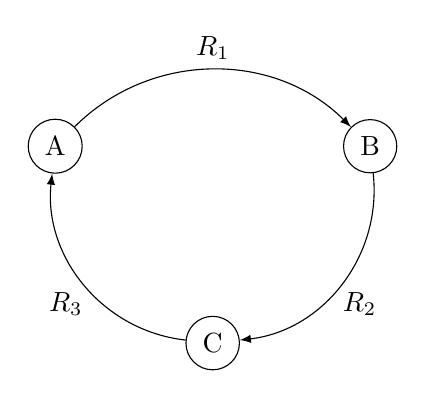
\begin{tikzpicture}
     \node [circle, draw] (A) at (-2,0) {A};
     \node [circle, draw] (B) at (2,0) {B};
     \node [circle, draw] (C) at (0,-2.5) {C};
     \draw[-latex] (A) to [bend left=45] node[above] {$R_1$} (B);
     \draw[-latex] (B) to [bend left=45] node[below = 10pt, pos=0.35] {$R_2$}(C);
     \draw[-latex] (C) to [bend left=45] node[below = 10pt, pos=0.65] {$R_3$}(A);
  \end{tikzpicture}
  \caption{Grafo Circular.}
  \label{fig:Circular}
\end{figure}

Este grafo a su vez tiene una representación en forma de matriz en la que cada columna representa una de las reacciones y cada fila un metabolito:

\begin{equation}
  \begin{matrix}
    & R_1 & R_2 & R_3\\
    A & -1 &  0 & +1\\
    B & +1 & -1 & 0\\
    C &  0 & +1 & -1\\
  \end{matrix}
\end{equation}

que se escribe:

\begin{equation}
  C = \begin{bmatrix}
  -1 &  0 & +1\\
  +1 & -1 & 0\\
  0 & +1 & -1\\
\end{bmatrix}
\end{equation}

\subsection{Flujos}
En la representación matricial descrita antes no mencionamos los flujos. Consideren la siguiente multiplicación:

\begin{equation}\label{eq:FluxMat}
  Cf =
  \begin{bmatrix}
  -1 &  0 & +1\\
  +1 & -1 & 0\\
  0 & +1 & -1\\
\end{bmatrix}
\begin{bmatrix} f_1\\ f_2\\ f_3\\ \end{bmatrix}
  =
f_1\begin{bmatrix} -1 \\ +1\\ 0 \end{bmatrix}
+ f_2\begin{bmatrix} 0\\ -1\\ +1 \end{bmatrix}
+ f_3\begin{bmatrix} +1\\ 0\\ -1 \end{bmatrix}
\end{equation}

Es una combinación lineal de las reacciones. Si $f_1 = 0$, etonces la reacción $R_1$ no se expresa. En ese sentido podemos pensar en $f_1, f_2, f_3$ como flujos en $R_1, R_2$ y $R_3$ respectivamente.

\par
El resultado de la multiplicación (\ref{eq:FluxMat}) tienen una interpretación interesante.  Si asociamos $A, B$ y $C$ a las filas $1, 2, 3$ entonces podemos escribir:

\begin{equation*}
  Cf =
  \begin{bmatrix}
     -f_1 + f_3\\
    f_1 - f_2\\
    f_2 - f_3
  \end{bmatrix} =
  \begin{bmatrix}
     \Delta A\\
     \Delta B\\
     \Delta C
  \end{bmatrix}
\end{equation*}

La multiplicación $Cf$ es cuanto cambió cada metabolito durante el flujo que atravezó el grafo.

El objetivo es especificar el vector de flujos para controlar el metabolismo. La única condición es que el vector de flujos seleccionado conserve la cantidad de metabolitos.

En términos matriciales buscamos los flujos que cumplen con la condición $SF = 0$. En el caso de la red circular~\ref{fig:Circular} los flujos permitdos son constantes com por ejemplo:

\begin{equation*}
  \begin{bmatrix}
     f_1\\
     f_2\\
     f_3
  \end{bmatrix} =
  \begin{bmatrix}
     2\\
     2\\
     2
  \end{bmatrix}
\end{equation*}



\section{Modelo Base y Vías Alternativas}

No existe una descripción del metabolismo de Sacaromises boulardii. La mayoría de los estudios usan el metabolismo de Sacaromises cerevisiae como una aproximación o como un modelo de base al que le añaden o le quitan racciones usando métodos computacionales para simular el metabolismo de S. boulardii. En este adoptamos la primera estrategia.

\par
El modelo de base es \emph{Saccharomyces cerevisiae S288C} que pueden encontrar en el siguiente enlace:

\begin{center}
  http://bigg.ucsd.edu/models/iMM904
\end{center}

\par
El modelo consta de aproximadamente $1200$ metabolitos que intervienen en mas de $1500$ reacciones reguladas por un poco mas de $900$ genes. Describen un red difícil de representar gráficamente.

\par

La producción de butirato no hace parte de este metabolismo. El primer objetivo es estudiar $4$ vías alternativas de producción de butirato:

\begin{table}[ht]
\begin{tabular}{cc}
genes & reaccciones \\
phaA & 2 acetyl-CoA → CoA + acetoacetyl-CoA \\
phaB & (R)-3-hydroxybutanoyl-CoA + NADP+ ↔ 3-acetoacetyl-CoA + NADPH + H+ \\
phaJ & (3R)-3-hydroxybutanoyl-CoA ↔ crotonoyl-CoA + H2O \\
Ter & crotonyl-CoA + NADH + H+ ↔ butyryl-CoA + NAD+ \\
TesB & butyryl-CoA + H2O → butyrate + CoA + H+
\end{tabular}
\caption{Modelo 1.}\label{tab:via1}
\end{table}



\begin{table}[ht]
\begin{tabular}{cc}
genes & reaccciones \\
phaA & 2 acetyl-CoA → CoA + acetoacetyl-CoA \\
phaBAv & (S)-3-hydroxybutanoyl-CoA + NAD+ ↔ 3-acetoacetyl-CoA + NADH + H+ \\
phaJ & (3R)-3-hydroxybutanoyl-CoA ↔ crotonoyl-CoA + H2O \\
Ter & crotonyl-CoA + NADH + H+ ↔ butyryl-CoA + NAD+ \\
TesB & butyryl-CoA + H2O → butyrate + CoA + H+
\end{tabular}
\caption{Modelo 1a.}\label{tab:via1a}
\end{table}


\begin{table}[ht]
\begin{tabular}{cc}
genes & reaccciones \\
phaA & 2 acetyl-CoA → CoA + acetoacetyl-CoA \\
phaBAv & (S)-3-hydroxybutanoyl-CoA + NAD+ ↔ 3-acetoacetyl-CoA + NADH + H+ \\
phaJ & (3S)-3-hydroxybutanoyl-CoA ↔ (E)-but-2enoyl-CoA + H2O \\
Ter & butanoyl-CoA + NAD+ ↔ (E)-but-2-enoyl-CoA + NADH + H+ \\
lvaE & ATP + Butanoate + CoA ↔ AMP + diphosphate + butanoyl-CoA
\end{tabular}
\caption{Modelo 2.}\label{tab:via2}
\end{table}


\begin{table}[ht]
\begin{tabular}{cc}
genes & reaction \\
phaA & 2 acetyl-CoA → CoA + acetoacetyl-CoA \\
phaBAv & (S)-3-hydroxybutanoyl-CoA + NAD+ ↔ 3-acetoacetyl-CoA + NADH + H+ \\
phaJ & (3S)-3-hydroxybutanoyl-CoA ↔ (E)-but-2enoyl-CoA + H2O \\
Ter & butanoyl-CoA + NAD+ ↔ (E)-but-2-enoyl-CoA + NADH + H+ \\
ptb & butanoyl-CoA + phosphate ↔  CoA + butanoyl phosphate \\
buk & ATP + butanoate ↔  ADP + butanoyl phosphate
\end{tabular}
\caption{Modelo 3.}\label{tab:via3}
\end{table}



El modelo de base de Sacaromises cerevisiae con las reacciones del cuadro:

\begin{itemize}
  \item \ref{tab:via1} es el modelo 1,
  \item \ref{tab:via1a} es el modelo 1a,
  \item \ref{tab:via2} es el modelo 2,
  \item \ref{tab:via3} es el modelo 3.
\end{itemize}

\subsection{Producción Butirato y Biomasa}

El metabolismo de cada uno de los modelos tiene un flujo que representa la biomasa en unidades $[1/h]$ y otro que representa la producción de butirato en unidades $[mmol/gdcw/h]$ que vamos a notar $f_{biomass}$ y $f_{but}$ respectivamente.

\par
El primer objetivo es describir la producción teorética de butirato y biomasas para cada modelo. Con este fin resolvemos:


\begin{equation*}\label{eq:prob1}
\begin{aligned}
& \underset{f}{\text{maximize}}
& &  f_{biomass} +  \lambda \ f_{but} \\
& \text{subject to}
& & Sf = 0 \\
&&& l_i \leq f_i \leq u_i, \; i = 1, \ldots, m.
\end{aligned}
\end{equation*}


La función obejetivo $f_{biomass} +  \lambda \ f_{but}$  es una combinación lineal de la biomasa y la producción de butirato. El número $\lambda$ es un parámetro que controla si el modelo produce mas biomasa o butirato. Por jemplo, cuando $\lambda = 0$, el metabolismo maximiza la producción de biomasa y cuando $\lambda = \infty $, el modelo maximiza la producción de butirato.

\par

Resolviendo el problema~(\ref{eq:prob1}) para $\lambda$ en $[0, 0.07]$ obtenemos las curvas de la figura (\ref{fig:paretoCurve}). En una curva cada punto representa un par $(f_{biomass}(\lambda), \ f_{but}(\lambda))$.


\begin{figure}[h]\label{fig:paretoCurve}
  \includegraphics{../plots/lambdaAllModelsAnn.png}
  \caption{Soluciones de (\ref{eq:prob1}) para $\lambda \in [0, 0.07]$.}
\end{figure}

Primero se puede notar que para cualquier producción de biomasa fija, los modelos $2$ y $3$ tienen una mayor producción de butirato.

Ademas si vemos los extremos de la curva correspondiente al modelo $2$, podemos notar que es capaz de producir la mayor cantidad de biomasa mientras sigue produciendo butirato y también produce la mayor cantidad de butirato sin dejar de producir biomasa.

\begin{center}
  ----------------------- FALTA INTUICION BIO -----------------------
\end{center}

\subsection{Producción en función de $o_2$ y $glucosa$}




\bibliographystyle{plain}
\bibliography{thebibliography}

\begin{thebibliography}{1}

\bibitem{python} Python Software Foundation. Python Language Reference, version 3.6 Available at http://www.python.org.

\bibitem{COBRApy} COBRApy: COnstraints-Based Reconstruction and Analysis for Python,
Ali Ebrahim, Joshua A. Lerman, Bernhard O. Palsson, and Daniel R. Hyduke,
BMC Systems Biology, 2013, 7:74.

\end{thebibliography}

\end{document}
This is never printed
